\documentclass[1p]{elsarticle_modified}
%\bibliographystyle{elsarticle-num}

%\usepackage[colorlinks]{hyperref}
%\usepackage{abbrmath_seonhwa} %\Abb, \Ascr, \Acal ,\Abf, \Afrak
\usepackage{amsfonts}
\usepackage{amssymb}
\usepackage{amsmath}
\usepackage{amsthm}
\usepackage{scalefnt}
\usepackage{amsbsy}
\usepackage{kotex}
\usepackage{caption}
\usepackage{subfig}
\usepackage{color}
\usepackage{graphicx}
\usepackage{xcolor} %% white, black, red, green, blue, cyan, magenta, yellow
\usepackage{float}
\usepackage{setspace}
\usepackage{hyperref}

\usepackage{tikz}
\usetikzlibrary{arrows}

\usepackage{multirow}
\usepackage{array} % fixed length table
\usepackage{hhline}

%%%%%%%%%%%%%%%%%%%%%
\makeatletter
\renewcommand*\env@matrix[1][\arraystretch]{%
	\edef\arraystretch{#1}%
	\hskip -\arraycolsep
	\let\@ifnextchar\new@ifnextchar
	\array{*\c@MaxMatrixCols c}}
\makeatother %https://tex.stackexchange.com/questions/14071/how-can-i-increase-the-line-spacing-in-a-matrix
%%%%%%%%%%%%%%%

\usepackage[normalem]{ulem}

\newcommand{\msout}[1]{\ifmmode\text{\sout{\ensuremath{#1}}}\else\sout{#1}\fi}
%SOURCE: \msout is \stkout macro in https://tex.stackexchange.com/questions/20609/strikeout-in-math-mode

\newcommand{\cancel}[1]{
	\ifmmode
	{\color{red}\msout{#1}}
	\else
	{\color{red}\sout{#1}}
	\fi
}

\newcommand{\add}[1]{
	{\color{blue}\uwave{#1}}
}

\newcommand{\replace}[2]{
	\ifmmode
	{\color{red}\msout{#1}}{\color{blue}\uwave{#2}}
	\else
	{\color{red}\sout{#1}}{\color{blue}\uwave{#2}}
	\fi
}

\newcommand{\Sol}{\mathcal{S}} %segment
\newcommand{\D}{D} %diagram
\newcommand{\A}{\mathcal{A}} %arc


%%%%%%%%%%%%%%%%%%%%%%%%%%%%%5 test

\def\sl{\operatorname{\textup{SL}}(2,\Cbb)}
\def\psl{\operatorname{\textup{PSL}}(2,\Cbb)}
\def\quan{\mkern 1mu \triangleright \mkern 1mu}

\theoremstyle{definition}
\newtheorem{thm}{Theorem}[section]
\newtheorem{prop}[thm]{Proposition}
\newtheorem{lem}[thm]{Lemma}
\newtheorem{ques}[thm]{Question}
\newtheorem{cor}[thm]{Corollary}
\newtheorem{defn}[thm]{Definition}
\newtheorem{exam}[thm]{Example}
\newtheorem{rmk}[thm]{Remark}
\newtheorem{alg}[thm]{Algorithm}

\newcommand{\I}{\sqrt{-1}}
\begin{document}

%\begin{frontmatter}
%
%\title{Boundary parabolic representations of knots up to 8 crossings}
%
%%% Group authors per affiliation:
%\author{Yunhi Cho} 
%\address{Department of Mathematics, University of Seoul, Seoul, Korea}
%\ead{yhcho@uos.ac.kr}
%
%
%\author{Seonhwa Kim} %\fnref{s_kim}}
%\address{Center for Geometry and Physics, Institute for Basic Science, Pohang, 37673, Korea}
%\ead{ryeona17@ibs.re.kr}
%
%\author{Hyuk Kim}
%\address{Department of Mathematical Sciences, Seoul National University, Seoul 08826, Korea}
%\ead{hyukkim@snu.ac.kr}
%
%\author{Seokbeom Yoon}
%\address{Department of Mathematical Sciences, Seoul National University, Seoul, 08826,  Korea}
%\ead{sbyoon15@snu.ac.kr}
%
%\begin{abstract}
%We find all boundary parabolic representation of knots up to 8 crossings.
%
%\end{abstract}
%\begin{keyword}
%    \MSC[2010] 57M25 
%\end{keyword}
%
%\end{frontmatter}

%\linenumbers
%\tableofcontents
%
\newcommand\colored[1]{\textcolor{white}{\rule[-0.35ex]{0.8em}{1.4ex}}\kern-0.8em\color{red} #1}%
%\newcommand\colored[1]{\textcolor{white}{ #1}\kern-2.17ex	\textcolor{white}{ #1}\kern-1.81ex	\textcolor{white}{ #1}\kern-2.15ex\color{red}#1	}

{\Large $\underline{11a_{282}~(K11a_{282})}$}

\setlength{\tabcolsep}{10pt}
\renewcommand{\arraystretch}{1.6}
\vspace{1cm}\begin{tabular}{m{100pt}>{\centering\arraybackslash}m{274pt}}
\multirow{5}{120pt}{
	\centering
	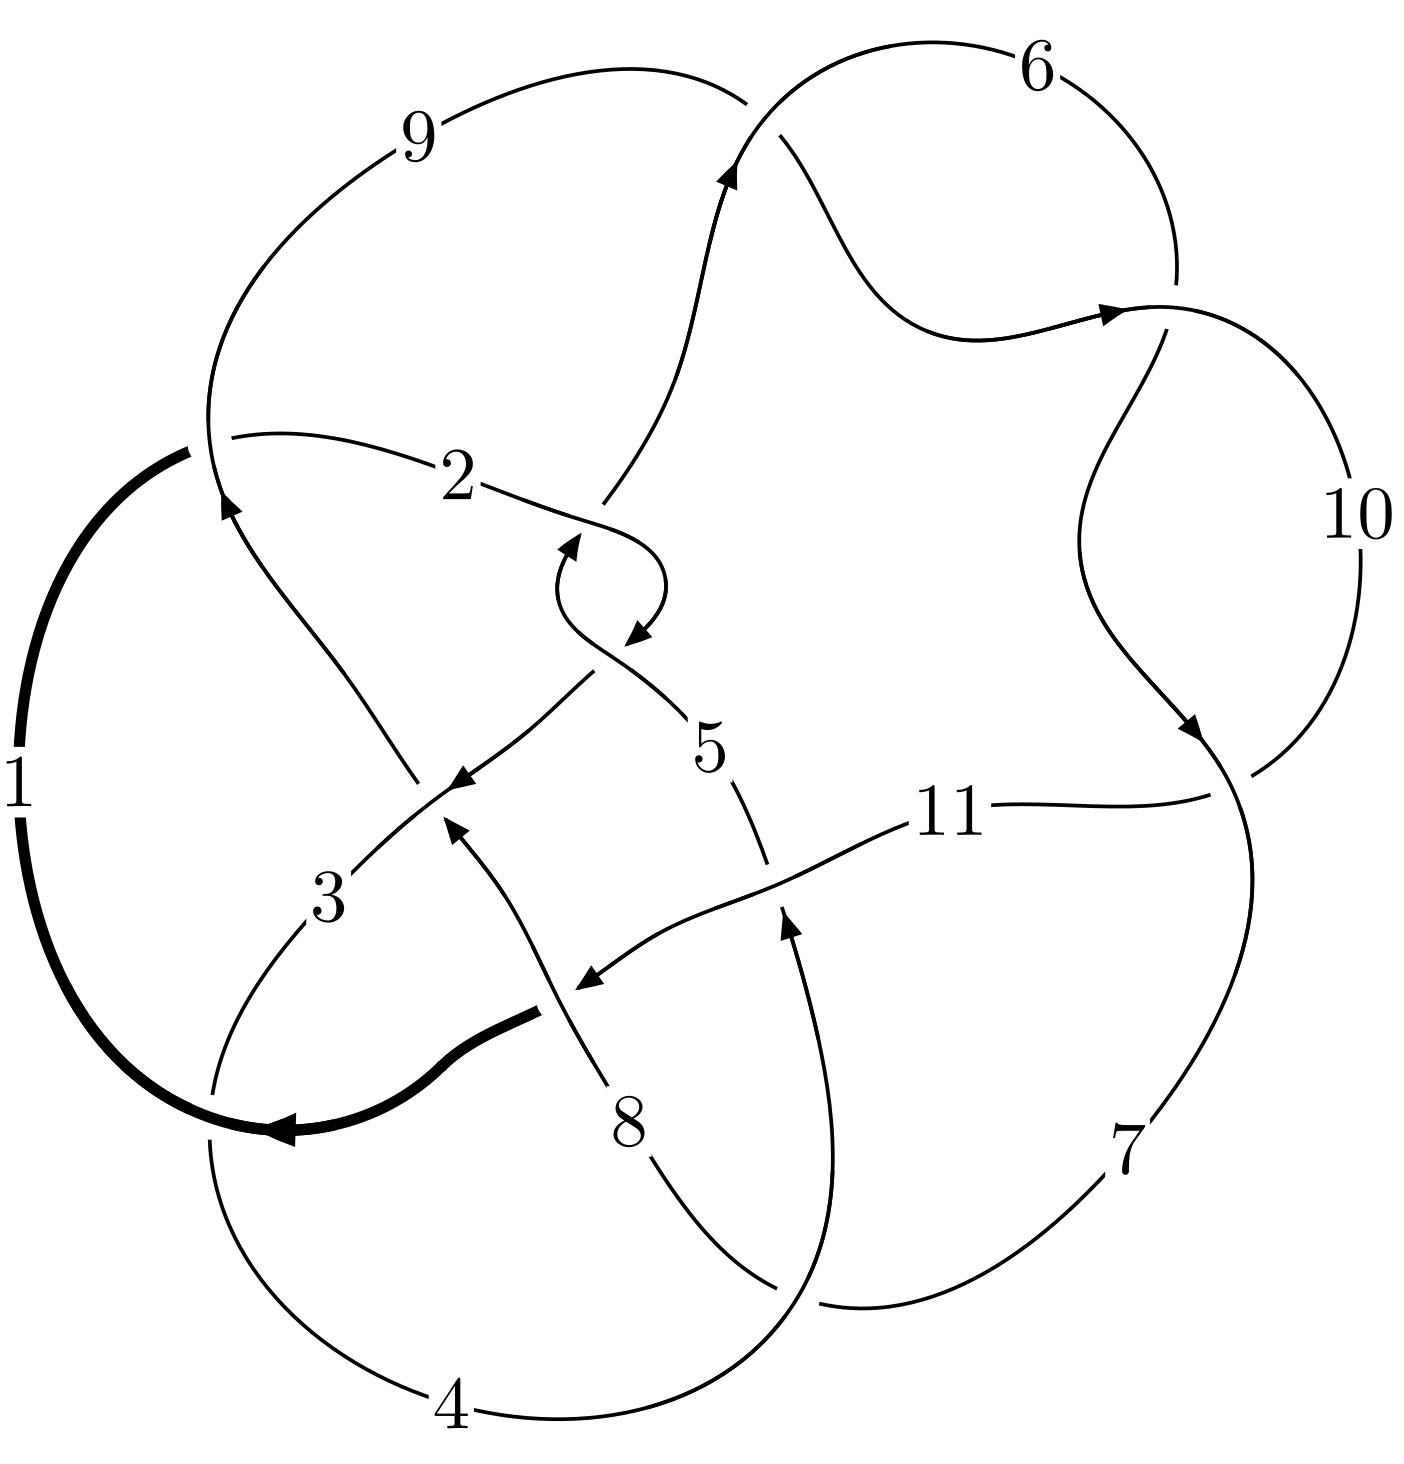
\includegraphics[width=112pt]{../../../GIT/diagram.site/Diagrams/png/531_11a_282.png}\\
\ \ \ A knot diagram\footnotemark}&
\allowdisplaybreaks
\textbf{Linearized knot diagam} \\
\cline{2-2}
 &
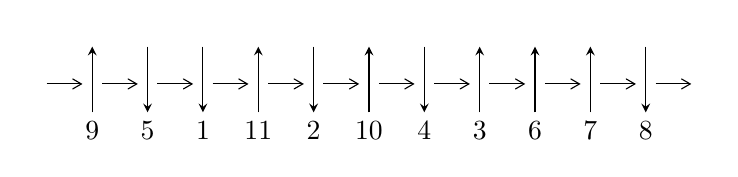
\begin{tikzpicture}[x=20pt, y=17pt]
	% nodes
	\node (C0) at (0, 0) {};
	\node (C1) at (1, 0) {};
	\node (C1U) at (1, +1) {};
	\node (C1D) at (1, -1) {9};

	\node (C2) at (2, 0) {};
	\node (C2U) at (2, +1) {};
	\node (C2D) at (2, -1) {5};

	\node (C3) at (3, 0) {};
	\node (C3U) at (3, +1) {};
	\node (C3D) at (3, -1) {1};

	\node (C4) at (4, 0) {};
	\node (C4U) at (4, +1) {};
	\node (C4D) at (4, -1) {11};

	\node (C5) at (5, 0) {};
	\node (C5U) at (5, +1) {};
	\node (C5D) at (5, -1) {2};

	\node (C6) at (6, 0) {};
	\node (C6U) at (6, +1) {};
	\node (C6D) at (6, -1) {10};

	\node (C7) at (7, 0) {};
	\node (C7U) at (7, +1) {};
	\node (C7D) at (7, -1) {4};

	\node (C8) at (8, 0) {};
	\node (C8U) at (8, +1) {};
	\node (C8D) at (8, -1) {3};

	\node (C9) at (9, 0) {};
	\node (C9U) at (9, +1) {};
	\node (C9D) at (9, -1) {6};

	\node (C10) at (10, 0) {};
	\node (C10U) at (10, +1) {};
	\node (C10D) at (10, -1) {7};

	\node (C11) at (11, 0) {};
	\node (C11U) at (11, +1) {};
	\node (C11D) at (11, -1) {8};
	\node (C12) at (12, 0) {};

	% arrows
	\draw[->,>={angle 60}]
	(C0) edge (C1) (C1) edge (C2) (C2) edge (C3) (C3) edge (C4) (C4) edge (C5) (C5) edge (C6) (C6) edge (C7) (C7) edge (C8) (C8) edge (C9) (C9) edge (C10) (C10) edge (C11) (C11) edge (C12) ;	\draw[->,>=stealth]
	(C1D) edge (C1U) (C2U) edge (C2D) (C3U) edge (C3D) (C4D) edge (C4U) (C5U) edge (C5D) (C6D) edge (C6U) (C7U) edge (C7D) (C8D) edge (C8U) (C9D) edge (C9U) (C10D) edge (C10U) (C11U) edge (C11D) ;
	\end{tikzpicture} \\
\hhline{~~} \\& 
\textbf{Solving Sequence} \\ \cline{2-2} 
 &
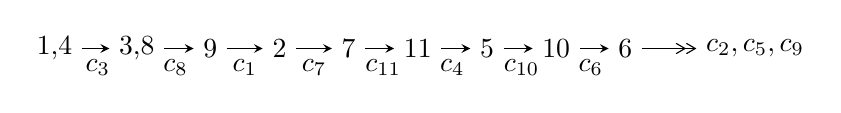
\begin{tikzpicture}[x=25pt, y=7pt]
	% node
	\node (A0) at (-1/8, 0) {1,4};
	\node (A1) at (17/16, 0) {3,8};
	\node (A2) at (17/8, 0) {9};
	\node (A3) at (25/8, 0) {2};
	\node (A4) at (33/8, 0) {7};
	\node (A5) at (41/8, 0) {11};
	\node (A6) at (49/8, 0) {5};
	\node (A7) at (57/8, 0) {10};
	\node (A8) at (65/8, 0) {6};
	\node (C1) at (1/2, -1) {$c_{3}$};
	\node (C2) at (13/8, -1) {$c_{8}$};
	\node (C3) at (21/8, -1) {$c_{1}$};
	\node (C4) at (29/8, -1) {$c_{7}$};
	\node (C5) at (37/8, -1) {$c_{11}$};
	\node (C6) at (45/8, -1) {$c_{4}$};
	\node (C7) at (53/8, -1) {$c_{10}$};
	\node (C8) at (61/8, -1) {$c_{6}$};
	\node (A9) at (10, 0) {$c_{2},c_{5},c_{9}$};

	% edge
	\draw[->,>=stealth]	
	(A0) edge (A1) (A1) edge (A2) (A2) edge (A3) (A3) edge (A4) (A4) edge (A5) (A5) edge (A6) (A6) edge (A7) (A7) edge (A8) ;
	\draw[->>,>={angle 60}]	
	(A8) edge (A9);
\end{tikzpicture} \\ 

\end{tabular} \\

\footnotetext{
The image of knot diagram is generated by the software ``\textbf{Draw programme}" developed by Andrew Bartholomew(\url{http://www.layer8.co.uk/maths/draw/index.htm\#Running-draw}), where we modified some parts for our purpose(\url{https://github.com/CATsTAILs/LinksPainter}).
}\phantom \\ \newline 
\centering \textbf{Ideals for irreducible components\footnotemark of $X_{\text{par}}$} 
 
\begin{align*}
I^u_{1}&=\langle 
2.13823\times10^{329} u^{79}-1.64855\times10^{330} u^{78}+\cdots+9.41459\times10^{329} b+1.13698\times10^{331},\\
\phantom{I^u_{1}}&\phantom{= \langle  }-1.24104\times10^{330} u^{79}+9.42225\times10^{330} u^{78}+\cdots+1.88292\times10^{330} a-8.31994\times10^{330},\\
\phantom{I^u_{1}}&\phantom{= \langle  }u^{80}-8 u^{79}+\cdots+232 u-16\rangle \\
I^u_{2}&=\langle 
3937680 u^{12}+7222127 u^{11}+\cdots+33692213 b+110970935,\\
\phantom{I^u_{2}}&\phantom{= \langle  }-33661342 u^{12}-112072005 u^{11}+\cdots+707536473 a-1914131674,\\
\phantom{I^u_{2}}&\phantom{= \langle  }u^{13}+3 u^{12}+u^{11}-5 u^{10}-10 u^9-11 u^8+21 u^6+22 u^5-5 u^4-6 u^3+32 u^2+49 u+21\rangle \\
\\
I^v_{1}&=\langle 
a,\;-6 v^3+4 v^2+5 b-33 v+13,\;v^4- v^3+6 v^2-4 v+1\rangle \\
\end{align*}
\raggedright * 3 irreducible components of $\dim_{\mathbb{C}}=0$, with total 97 representations.\\
\footnotetext{All coefficients of polynomials are rational numbers. But the coefficients are sometimes approximated in decimal forms when there is not enough margin.}
\newpage
\renewcommand{\arraystretch}{1}
\centering \section*{I. $I^u_{1}= \langle 2.14\times10^{329} u^{79}-1.65\times10^{330} u^{78}+\cdots+9.41\times10^{329} b+1.14\times10^{331},\;-1.24\times10^{330} u^{79}+9.42\times10^{330} u^{78}+\cdots+1.88\times10^{330} a-8.32\times10^{330},\;u^{80}-8 u^{79}+\cdots+232 u-16 \rangle$}
\flushleft \textbf{(i) Arc colorings}\\
\begin{tabular}{m{7pt} m{180pt} m{7pt} m{180pt} }
\flushright $a_{1}=$&$\begin{pmatrix}0\\u\end{pmatrix}$ \\
\flushright $a_{4}=$&$\begin{pmatrix}1\\0\end{pmatrix}$ \\
\flushright $a_{3}=$&$\begin{pmatrix}1\\- u^2\end{pmatrix}$ \\
\flushright $a_{8}=$&$\begin{pmatrix}0.659106 u^{79}-5.00407 u^{78}+\cdots-122.616 u+4.41864\\-0.227119 u^{79}+1.75106 u^{78}+\cdots+151.411 u-12.0768\end{pmatrix}$ \\
\flushright $a_{9}=$&$\begin{pmatrix}0.472695 u^{79}-3.57754 u^{78}+\cdots-23.0170 u-3.35768\\-0.204660 u^{79}+1.57688 u^{78}+\cdots+139.369 u-11.0407\end{pmatrix}$ \\
\flushright $a_{2}=$&$\begin{pmatrix}0.191836 u^{79}-1.57834 u^{78}+\cdots-74.5281 u+7.17744\\0.252449 u^{79}-1.90962 u^{78}+\cdots-23.3077 u+1.27382\end{pmatrix}$ \\
\flushright $a_{7}=$&$\begin{pmatrix}0.431988 u^{79}-3.25301 u^{78}+\cdots+28.7946 u-7.65818\\-0.227119 u^{79}+1.75106 u^{78}+\cdots+151.411 u-12.0768\end{pmatrix}$ \\
\flushright $a_{11}=$&$\begin{pmatrix}-0.108601 u^{79}+0.694864 u^{78}+\cdots-42.0396 u+5.25398\\0.251916 u^{79}-1.93686 u^{78}+\cdots-58.9949 u+4.13119\end{pmatrix}$ \\
\flushright $a_{5}=$&$\begin{pmatrix}-0.0246729 u^{79}+0.192222 u^{78}+\cdots+0.535696 u-3.21204\\-0.255007 u^{79}+1.91467 u^{78}+\cdots+51.6752 u-3.40150\end{pmatrix}$ \\
\flushright $a_{10}=$&$\begin{pmatrix}0.223539 u^{79}-1.88491 u^{78}+\cdots-80.6924 u+6.78770\\0.436133 u^{79}-3.33065 u^{78}+\cdots-70.4389 u+4.43414\end{pmatrix}$ \\
\flushright $a_{6}=$&$\begin{pmatrix}-0.0921991 u^{79}+0.895913 u^{78}+\cdots+43.4256 u-3.45099\\-0.411264 u^{79}+3.14443 u^{78}+\cdots+63.0579 u-3.81043\end{pmatrix}$\\ \flushright $a_{6}=$&$\begin{pmatrix}-0.0921991 u^{79}+0.895913 u^{78}+\cdots+43.4256 u-3.45099\\-0.411264 u^{79}+3.14443 u^{78}+\cdots+63.0579 u-3.81043\end{pmatrix}$\\&\end{tabular}
\flushleft \textbf{(ii) Obstruction class $= -1$}\\~\\
\flushleft \textbf{(iii) Cusp Shapes $= -0.662366 u^{79}+5.15267 u^{78}+\cdots+112.853 u-7.98177$}\\~\\
\newpage\renewcommand{\arraystretch}{1}
\flushleft \textbf{(iv) u-Polynomials at the component}\newline \\
\begin{tabular}{m{50pt}|m{274pt}}
Crossings & \hspace{64pt}u-Polynomials at each crossing \\
\hline $$\begin{aligned}c_{1}\end{aligned}$$&$\begin{aligned}
&u^{80}- u^{79}+\cdots+166862 u+35227
\end{aligned}$\\
\hline $$\begin{aligned}c_{2},c_{5}\end{aligned}$$&$\begin{aligned}
&u^{80}+3 u^{79}+\cdots+537 u+55
\end{aligned}$\\
\hline $$\begin{aligned}c_{3}\end{aligned}$$&$\begin{aligned}
&u^{80}-8 u^{79}+\cdots+232 u-16
\end{aligned}$\\
\hline $$\begin{aligned}c_{4}\end{aligned}$$&$\begin{aligned}
&u^{80}-3 u^{79}+\cdots-1033 u-173
\end{aligned}$\\
\hline $$\begin{aligned}c_{6},c_{9},c_{10}\end{aligned}$$&$\begin{aligned}
&u^{80}-3 u^{79}+\cdots+34 u+1
\end{aligned}$\\
\hline $$\begin{aligned}c_{7}\end{aligned}$$&$\begin{aligned}
&u^{80}+3 u^{79}+\cdots+357 u-319
\end{aligned}$\\
\hline $$\begin{aligned}c_{8}\end{aligned}$$&$\begin{aligned}
&u^{80}+3 u^{78}+\cdots+26 u+1
\end{aligned}$\\
\hline $$\begin{aligned}c_{11}\end{aligned}$$&$\begin{aligned}
&u^{80}-2 u^{79}+\cdots+28 u+5
\end{aligned}$\\
\hline
\end{tabular}\\~\\
\newpage\renewcommand{\arraystretch}{1}
\flushleft \textbf{(v) Riley Polynomials at the component}\newline \\
\begin{tabular}{m{50pt}|m{274pt}}
Crossings & \hspace{64pt}Riley Polynomials at each crossing \\
\hline $$\begin{aligned}c_{1}\end{aligned}$$&$\begin{aligned}
&y^{80}-37 y^{79}+\cdots-40557549062 y+1240941529
\end{aligned}$\\
\hline $$\begin{aligned}c_{2},c_{5}\end{aligned}$$&$\begin{aligned}
&y^{80}+55 y^{79}+\cdots-597359 y+3025
\end{aligned}$\\
\hline $$\begin{aligned}c_{3}\end{aligned}$$&$\begin{aligned}
&y^{80}+8 y^{79}+\cdots+1728 y+256
\end{aligned}$\\
\hline $$\begin{aligned}c_{4}\end{aligned}$$&$\begin{aligned}
&y^{80}-23 y^{79}+\cdots-1094423 y+29929
\end{aligned}$\\
\hline $$\begin{aligned}c_{6},c_{9},c_{10}\end{aligned}$$&$\begin{aligned}
&y^{80}-91 y^{79}+\cdots-880 y+1
\end{aligned}$\\
\hline $$\begin{aligned}c_{7}\end{aligned}$$&$\begin{aligned}
&y^{80}+19 y^{79}+\cdots+3233535 y+101761
\end{aligned}$\\
\hline $$\begin{aligned}c_{8}\end{aligned}$$&$\begin{aligned}
&y^{80}+6 y^{79}+\cdots-284 y+1
\end{aligned}$\\
\hline $$\begin{aligned}c_{11}\end{aligned}$$&$\begin{aligned}
&y^{80}-12 y^{79}+\cdots-614 y+25
\end{aligned}$\\
\hline
\end{tabular}\\~\\
\newpage\flushleft \textbf{(vi) Complex Volumes and Cusp Shapes}
$$\begin{array}{c|c|c}  
\text{Solutions to }I^u_{1}& \I (\text{vol} + \sqrt{-1}CS) & \text{Cusp shape}\\
 \hline 
\begin{aligned}
u &= \phantom{-}0.840683 + 0.530658 I \\
a &= \phantom{-}1.35694 + 0.42194 I \\
b &= -0.649032 - 1.118120 I\end{aligned}
 & \phantom{-}4.67943 - 5.53958 I & \phantom{-0.000000 } 0 \\ \hline\begin{aligned}
u &= \phantom{-}0.840683 - 0.530658 I \\
a &= \phantom{-}1.35694 - 0.42194 I \\
b &= -0.649032 + 1.118120 I\end{aligned}
 & \phantom{-}4.67943 + 5.53958 I & \phantom{-0.000000 } 0 \\ \hline\begin{aligned}
u &= \phantom{-}0.180021 + 0.949720 I \\
a &= -0.367561 + 0.226099 I \\
b &= \phantom{-}0.495810 - 1.018400 I\end{aligned}
 & \phantom{-}2.87404 - 1.12286 I & \phantom{-0.000000 } 0 \\ \hline\begin{aligned}
u &= \phantom{-}0.180021 - 0.949720 I \\
a &= -0.367561 - 0.226099 I \\
b &= \phantom{-}0.495810 + 1.018400 I\end{aligned}
 & \phantom{-}2.87404 + 1.12286 I & \phantom{-0.000000 } 0 \\ \hline\begin{aligned}
u &= -0.104754 + 0.947386 I \\
a &= -1.019370 + 0.771877 I \\
b &= -0.275736 + 0.979574 I\end{aligned}
 & \phantom{-}8.07177 + 3.14572 I & \phantom{-0.000000 } 0 \\ \hline\begin{aligned}
u &= -0.104754 - 0.947386 I \\
a &= -1.019370 - 0.771877 I \\
b &= -0.275736 - 0.979574 I\end{aligned}
 & \phantom{-}8.07177 - 3.14572 I & \phantom{-0.000000 } 0 \\ \hline\begin{aligned}
u &= \phantom{-}0.661970 + 0.670152 I \\
a &= \phantom{-}0.630442 - 0.139375 I \\
b &= -1.31406 + 0.69854 I\end{aligned}
 & \phantom{-}2.00824 - 5.11347 I & \phantom{-0.000000 } 0 \\ \hline\begin{aligned}
u &= \phantom{-}0.661970 - 0.670152 I \\
a &= \phantom{-}0.630442 + 0.139375 I \\
b &= -1.31406 - 0.69854 I\end{aligned}
 & \phantom{-}2.00824 + 5.11347 I & \phantom{-0.000000 } 0 \\ \hline\begin{aligned}
u &= -0.892356 + 0.677258 I \\
a &= \phantom{-}1.379940 - 0.203911 I \\
b &= -0.493046 + 0.873919 I\end{aligned}
 & \phantom{-}0.18057 + 4.85137 I & \phantom{-0.000000 } 0 \\ \hline\begin{aligned}
u &= -0.892356 - 0.677258 I \\
a &= \phantom{-}1.379940 + 0.203911 I \\
b &= -0.493046 - 0.873919 I\end{aligned}
 & \phantom{-}0.18057 - 4.85137 I & \phantom{-0.000000 } 0\\
 \hline 
 \end{array}$$\newpage$$\begin{array}{c|c|c}  
\text{Solutions to }I^u_{1}& \I (\text{vol} + \sqrt{-1}CS) & \text{Cusp shape}\\
 \hline 
\begin{aligned}
u &= \phantom{-}0.985954 + 0.565348 I \\
a &= -0.680804 + 0.032647 I \\
b &= \phantom{-}1.90069 - 0.40869 I\end{aligned}
 & \phantom{-}8.36747 - 7.88982 I & \phantom{-0.000000 } 0 \\ \hline\begin{aligned}
u &= \phantom{-}0.985954 - 0.565348 I \\
a &= -0.680804 - 0.032647 I \\
b &= \phantom{-}1.90069 + 0.40869 I\end{aligned}
 & \phantom{-}8.36747 + 7.88982 I & \phantom{-0.000000 } 0 \\ \hline\begin{aligned}
u &= -0.123573 + 0.830325 I \\
a &= -1.204170 - 0.462968 I \\
b &= \phantom{-}0.94407 - 1.46088 I\end{aligned}
 & \phantom{-}12.6911 + 7.3736 I & \phantom{-}10.17010 - 5.87052 I \\ \hline\begin{aligned}
u &= -0.123573 - 0.830325 I \\
a &= -1.204170 + 0.462968 I \\
b &= \phantom{-}0.94407 + 1.46088 I\end{aligned}
 & \phantom{-}12.6911 - 7.3736 I & \phantom{-}10.17010 + 5.87052 I \\ \hline\begin{aligned}
u &= -1.099290 + 0.392496 I \\
a &= -0.452143 - 0.129794 I \\
b &= \phantom{-}1.013660 + 0.291391 I\end{aligned}
 & -2.29379 + 0.10630 I & \phantom{-0.000000 } 0 \\ \hline\begin{aligned}
u &= -1.099290 - 0.392496 I \\
a &= -0.452143 + 0.129794 I \\
b &= \phantom{-}1.013660 - 0.291391 I\end{aligned}
 & -2.29379 - 0.10630 I & \phantom{-0.000000 } 0 \\ \hline\begin{aligned}
u &= \phantom{-}0.306099 + 0.749139 I \\
a &= \phantom{-}1.17339 + 1.71227 I \\
b &= \phantom{-}0.307186 + 0.932817 I\end{aligned}
 & \phantom{-}12.2687 - 8.2177 I & \phantom{-}9.86670 + 6.29220 I \\ \hline\begin{aligned}
u &= \phantom{-}0.306099 - 0.749139 I \\
a &= \phantom{-}1.17339 - 1.71227 I \\
b &= \phantom{-}0.307186 - 0.932817 I\end{aligned}
 & \phantom{-}12.2687 + 8.2177 I & \phantom{-}9.86670 - 6.29220 I \\ \hline\begin{aligned}
u &= -0.694646 + 0.970578 I \\
a &= \phantom{-}0.528065 + 0.382905 I \\
b &= -0.464932 + 0.052795 I\end{aligned}
 & -1.04673 + 2.15724 I & \phantom{-0.000000 } 0 \\ \hline\begin{aligned}
u &= -0.694646 - 0.970578 I \\
a &= \phantom{-}0.528065 - 0.382905 I \\
b &= -0.464932 - 0.052795 I\end{aligned}
 & -1.04673 - 2.15724 I & \phantom{-0.000000 } 0\\
 \hline 
 \end{array}$$\newpage$$\begin{array}{c|c|c}  
\text{Solutions to }I^u_{1}& \I (\text{vol} + \sqrt{-1}CS) & \text{Cusp shape}\\
 \hline 
\begin{aligned}
u &= -1.24309\phantom{ +0.000000I} \\
a &= \phantom{-}0.562759\phantom{ +0.000000I} \\
b &= -2.26176\phantom{ +0.000000I}\end{aligned}
 & \phantom{-}2.97554\phantom{ +0.000000I} & \phantom{-0.000000 } 0 \\ \hline\begin{aligned}
u &= -0.237050 + 0.708818 I \\
a &= -1.70391 - 1.51624 I \\
b &= \phantom{-}0.096962 - 0.807799 I\end{aligned}
 & \phantom{-}2.27021 + 2.30399 I & \phantom{-}10.35821 - 6.17851 I \\ \hline\begin{aligned}
u &= -0.237050 - 0.708818 I \\
a &= -1.70391 + 1.51624 I \\
b &= \phantom{-}0.096962 + 0.807799 I\end{aligned}
 & \phantom{-}2.27021 - 2.30399 I & \phantom{-}10.35821 + 6.17851 I \\ \hline\begin{aligned}
u &= \phantom{-}0.542023 + 1.130380 I \\
a &= -1.275280 + 0.501763 I \\
b &= \phantom{-}0.686902 + 0.769875 I\end{aligned}
 & \phantom{-}2.03522 - 6.05720 I & \phantom{-0.000000 } 0 \\ \hline\begin{aligned}
u &= \phantom{-}0.542023 - 1.130380 I \\
a &= -1.275280 - 0.501763 I \\
b &= \phantom{-}0.686902 - 0.769875 I\end{aligned}
 & \phantom{-}2.03522 + 6.05720 I & \phantom{-0.000000 } 0 \\ \hline\begin{aligned}
u &= \phantom{-}0.600098 + 0.443545 I \\
a &= -1.68558 - 0.03962 I \\
b &= \phantom{-}0.580481 + 0.881463 I\end{aligned}
 & -0.19438 - 2.30796 I & -0.22105 + 1.92438 I \\ \hline\begin{aligned}
u &= \phantom{-}0.600098 - 0.443545 I \\
a &= -1.68558 + 0.03962 I \\
b &= \phantom{-}0.580481 - 0.881463 I\end{aligned}
 & -0.19438 + 2.30796 I & -0.22105 - 1.92438 I \\ \hline\begin{aligned}
u &= -1.25520\phantom{ +0.000000I} \\
a &= -0.463800\phantom{ +0.000000I} \\
b &= \phantom{-}1.40127\phantom{ +0.000000I}\end{aligned}
 & -2.39628\phantom{ +0.000000I} & \phantom{-0.000000 } 0 \\ \hline\begin{aligned}
u &= \phantom{-}0.031843 + 0.737888 I \\
a &= \phantom{-}1.61286 + 0.51963 I \\
b &= -0.793415 + 0.882844 I\end{aligned}
 & \phantom{-}4.86209 + 2.93048 I & \phantom{-}10.03952 - 4.02142 I \\ \hline\begin{aligned}
u &= \phantom{-}0.031843 - 0.737888 I \\
a &= \phantom{-}1.61286 - 0.51963 I \\
b &= -0.793415 - 0.882844 I\end{aligned}
 & \phantom{-}4.86209 - 2.93048 I & \phantom{-}10.03952 + 4.02142 I\\
 \hline 
 \end{array}$$\newpage$$\begin{array}{c|c|c}  
\text{Solutions to }I^u_{1}& \I (\text{vol} + \sqrt{-1}CS) & \text{Cusp shape}\\
 \hline 
\begin{aligned}
u &= \phantom{-}0.134268 + 0.711933 I \\
a &= -1.92090 - 1.34681 I \\
b &= \phantom{-}0.091092 - 0.685075 I\end{aligned}
 & \phantom{-}4.72557 - 3.64290 I & \phantom{-}11.77697 + 3.87111 I \\ \hline\begin{aligned}
u &= \phantom{-}0.134268 - 0.711933 I \\
a &= -1.92090 + 1.34681 I \\
b &= \phantom{-}0.091092 + 0.685075 I\end{aligned}
 & \phantom{-}4.72557 + 3.64290 I & \phantom{-}11.77697 - 3.87111 I \\ \hline\begin{aligned}
u &= -0.773109 + 1.021590 I \\
a &= \phantom{-}1.037650 + 0.280309 I \\
b &= -0.636257 + 0.699388 I\end{aligned}
 & -0.70494 + 3.55934 I & \phantom{-0.000000 } 0 \\ \hline\begin{aligned}
u &= -0.773109 - 1.021590 I \\
a &= \phantom{-}1.037650 - 0.280309 I \\
b &= -0.636257 - 0.699388 I\end{aligned}
 & -0.70494 - 3.55934 I & \phantom{-0.000000 } 0 \\ \hline\begin{aligned}
u &= \phantom{-}0.503388 + 0.507249 I \\
a &= \phantom{-}1.49012 - 1.24386 I \\
b &= -0.436495 - 0.728628 I\end{aligned}
 & \phantom{-}2.29106 + 1.38243 I & \phantom{-}5.34088 + 2.43199 I \\ \hline\begin{aligned}
u &= \phantom{-}0.503388 - 0.507249 I \\
a &= \phantom{-}1.49012 + 1.24386 I \\
b &= -0.436495 + 0.728628 I\end{aligned}
 & \phantom{-}2.29106 - 1.38243 I & \phantom{-}5.34088 - 2.43199 I \\ \hline\begin{aligned}
u &= -0.618698 + 0.202823 I \\
a &= -1.75964 + 0.57403 I \\
b &= \phantom{-}0.882942 + 0.636078 I\end{aligned}
 & \phantom{-}5.11206 + 0.66852 I & \phantom{-}4.43405 - 0.97778 I \\ \hline\begin{aligned}
u &= -0.618698 - 0.202823 I \\
a &= -1.75964 - 0.57403 I \\
b &= \phantom{-}0.882942 - 0.636078 I\end{aligned}
 & \phantom{-}5.11206 - 0.66852 I & \phantom{-}4.43405 + 0.97778 I \\ \hline\begin{aligned}
u &= \phantom{-}0.037653 + 1.353780 I \\
a &= \phantom{-}0.50667 - 1.33040 I \\
b &= -0.007936 - 0.628942 I\end{aligned}
 & \phantom{-}9.22965 + 1.15849 I & \phantom{-0.000000 } 0 \\ \hline\begin{aligned}
u &= \phantom{-}0.037653 - 1.353780 I \\
a &= \phantom{-}0.50667 + 1.33040 I \\
b &= -0.007936 + 0.628942 I\end{aligned}
 & \phantom{-}9.22965 - 1.15849 I & \phantom{-0.000000 } 0\\
 \hline 
 \end{array}$$\newpage$$\begin{array}{c|c|c}  
\text{Solutions to }I^u_{1}& \I (\text{vol} + \sqrt{-1}CS) & \text{Cusp shape}\\
 \hline 
\begin{aligned}
u &= -0.606329 + 0.168371 I \\
a &= \phantom{-}0.448090 + 0.339379 I \\
b &= -0.90226 - 1.37943 I\end{aligned}
 & \phantom{-}1.23578 - 1.64636 I & -4.64141 + 0.02219 I \\ \hline\begin{aligned}
u &= -0.606329 - 0.168371 I \\
a &= \phantom{-}0.448090 - 0.339379 I \\
b &= -0.90226 + 1.37943 I\end{aligned}
 & \phantom{-}1.23578 + 1.64636 I & -4.64141 - 0.02219 I \\ \hline\begin{aligned}
u &= \phantom{-}0.391328 + 1.322250 I \\
a &= \phantom{-}0.119458 + 0.817321 I \\
b &= \phantom{-}0.388099 + 1.137900 I\end{aligned}
 & \phantom{-}11.34390 + 2.19538 I & \phantom{-0.000000 } 0 \\ \hline\begin{aligned}
u &= \phantom{-}0.391328 - 1.322250 I \\
a &= \phantom{-}0.119458 - 0.817321 I \\
b &= \phantom{-}0.388099 - 1.137900 I\end{aligned}
 & \phantom{-}11.34390 - 2.19538 I & \phantom{-0.000000 } 0 \\ \hline\begin{aligned}
u &= -1.27792 + 0.61735 I \\
a &= -0.960577 + 0.453365 I \\
b &= \phantom{-}0.688710 - 1.026030 I\end{aligned}
 & \phantom{-}6.33830 + 6.39761 I & \phantom{-0.000000 } 0 \\ \hline\begin{aligned}
u &= -1.27792 - 0.61735 I \\
a &= -0.960577 - 0.453365 I \\
b &= \phantom{-}0.688710 + 1.026030 I\end{aligned}
 & \phantom{-}6.33830 - 6.39761 I & \phantom{-0.000000 } 0 \\ \hline\begin{aligned}
u &= \phantom{-}0.032952 + 0.576655 I \\
a &= \phantom{-}1.46468 - 0.71797 I \\
b &= -0.101802 - 0.683648 I\end{aligned}
 & \phantom{-}1.19697 + 0.93213 I & \phantom{-}5.66000 - 4.34612 I \\ \hline\begin{aligned}
u &= \phantom{-}0.032952 - 0.576655 I \\
a &= \phantom{-}1.46468 + 0.71797 I \\
b &= -0.101802 + 0.683648 I\end{aligned}
 & \phantom{-}1.19697 - 0.93213 I & \phantom{-}5.66000 + 4.34612 I \\ \hline\begin{aligned}
u &= \phantom{-}0.95738 + 1.05845 I \\
a &= \phantom{-}0.724741 + 0.037351 I \\
b &= -0.848862 - 0.953885 I\end{aligned}
 & \phantom{-}4.89732 - 3.26135 I & \phantom{-0.000000 } 0 \\ \hline\begin{aligned}
u &= \phantom{-}0.95738 - 1.05845 I \\
a &= \phantom{-}0.724741 - 0.037351 I \\
b &= -0.848862 + 0.953885 I\end{aligned}
 & \phantom{-}4.89732 + 3.26135 I & \phantom{-0.000000 } 0\\
 \hline 
 \end{array}$$\newpage$$\begin{array}{c|c|c}  
\text{Solutions to }I^u_{1}& \I (\text{vol} + \sqrt{-1}CS) & \text{Cusp shape}\\
 \hline 
\begin{aligned}
u &= \phantom{-}1.31711 + 0.58795 I \\
a &= \phantom{-}0.317199 - 0.365878 I \\
b &= -0.650343 + 0.545302 I\end{aligned}
 & \phantom{-}1.32833 + 5.02960 I & \phantom{-0.000000 } 0 \\ \hline\begin{aligned}
u &= \phantom{-}1.31711 - 0.58795 I \\
a &= \phantom{-}0.317199 + 0.365878 I \\
b &= -0.650343 - 0.545302 I\end{aligned}
 & \phantom{-}1.32833 - 5.02960 I & \phantom{-0.000000 } 0 \\ \hline\begin{aligned}
u &= -0.91120 + 1.16270 I \\
a &= -0.915353 - 0.231344 I \\
b &= \phantom{-}0.867163 - 1.107560 I\end{aligned}
 & -0.36262 + 7.36216 I & \phantom{-0.000000 } 0 \\ \hline\begin{aligned}
u &= -0.91120 - 1.16270 I \\
a &= -0.915353 + 0.231344 I \\
b &= \phantom{-}0.867163 + 1.107560 I\end{aligned}
 & -0.36262 - 7.36216 I & \phantom{-0.000000 } 0 \\ \hline\begin{aligned}
u &= \phantom{-}0.84233 + 1.21734 I \\
a &= \phantom{-}1.048000 - 0.255925 I \\
b &= -0.861274 - 1.103910 I\end{aligned}
 & \phantom{-}3.36104 - 12.42420 I & \phantom{-0.000000 } 0 \\ \hline\begin{aligned}
u &= \phantom{-}0.84233 - 1.21734 I \\
a &= \phantom{-}1.048000 + 0.255925 I \\
b &= -0.861274 + 1.103910 I\end{aligned}
 & \phantom{-}3.36104 + 12.42420 I & \phantom{-0.000000 } 0 \\ \hline\begin{aligned}
u &= \phantom{-}0.090035 + 0.437599 I \\
a &= \phantom{-}1.30433 - 1.91862 I \\
b &= -0.33747 - 1.70963 I\end{aligned}
 & \phantom{-}5.32179 - 3.40594 I & \phantom{-}2.62572 + 4.19099 I \\ \hline\begin{aligned}
u &= \phantom{-}0.090035 - 0.437599 I \\
a &= \phantom{-}1.30433 + 1.91862 I \\
b &= -0.33747 + 1.70963 I\end{aligned}
 & \phantom{-}5.32179 + 3.40594 I & \phantom{-}2.62572 - 4.19099 I \\ \hline\begin{aligned}
u &= \phantom{-}0.97937 + 1.22317 I \\
a &= -0.701705 + 0.073709 I \\
b &= \phantom{-}1.12921 + 1.37276 I\end{aligned}
 & \phantom{-}12.19820 - 2.98748 I & \phantom{-0.000000 } 0 \\ \hline\begin{aligned}
u &= \phantom{-}0.97937 - 1.22317 I \\
a &= -0.701705 - 0.073709 I \\
b &= \phantom{-}1.12921 - 1.37276 I\end{aligned}
 & \phantom{-}12.19820 + 2.98748 I & \phantom{-0.000000 } 0\\
 \hline 
 \end{array}$$\newpage$$\begin{array}{c|c|c}  
\text{Solutions to }I^u_{1}& \I (\text{vol} + \sqrt{-1}CS) & \text{Cusp shape}\\
 \hline 
\begin{aligned}
u &= \phantom{-}1.10845 + 1.13168 I \\
a &= -0.556064 - 0.215884 I \\
b &= \phantom{-}0.231975 + 0.619801 I\end{aligned}
 & \phantom{-}4.41415 - 4.62933 I & \phantom{-0.000000 } 0 \\ \hline\begin{aligned}
u &= \phantom{-}1.10845 - 1.13168 I \\
a &= -0.556064 + 0.215884 I \\
b &= \phantom{-}0.231975 - 0.619801 I\end{aligned}
 & \phantom{-}4.41415 + 4.62933 I & \phantom{-0.000000 } 0 \\ \hline\begin{aligned}
u &= -0.62097 + 1.48212 I \\
a &= -0.603775 - 0.282250 I \\
b &= -0.083111 - 0.634277 I\end{aligned}
 & \phantom{-}6.44646 + 1.55360 I & \phantom{-0.000000 } 0 \\ \hline\begin{aligned}
u &= -0.62097 - 1.48212 I \\
a &= -0.603775 + 0.282250 I \\
b &= -0.083111 + 0.634277 I\end{aligned}
 & \phantom{-}6.44646 - 1.55360 I & \phantom{-0.000000 } 0 \\ \hline\begin{aligned}
u &= -0.22286 + 1.62378 I \\
a &= \phantom{-}0.179632 - 0.083745 I \\
b &= \phantom{-}0.047288 + 0.965549 I\end{aligned}
 & \phantom{-}10.69120 + 0.96957 I & \phantom{-0.000000 } 0 \\ \hline\begin{aligned}
u &= -0.22286 - 1.62378 I \\
a &= \phantom{-}0.179632 + 0.083745 I \\
b &= \phantom{-}0.047288 - 0.965549 I\end{aligned}
 & \phantom{-}10.69120 - 0.96957 I & \phantom{-0.000000 } 0 \\ \hline\begin{aligned}
u &= \phantom{-}0.358983\phantom{ +0.000000I} \\
a &= \phantom{-}2.21477\phantom{ +0.000000I} \\
b &= -0.931576\phantom{ +0.000000I}\end{aligned}
 & \phantom{-}1.95889\phantom{ +0.000000I} & \phantom{-}7.65550\phantom{ +0.000000I} \\ \hline\begin{aligned}
u &= \phantom{-}0.194090 + 0.272092 I \\
a &= -0.20112 + 2.73214 I \\
b &= \phantom{-}0.150945 - 0.683093 I\end{aligned}
 & -0.19507 + 1.98978 I & -2.02649 - 3.13292 I \\ \hline\begin{aligned}
u &= \phantom{-}0.194090 - 0.272092 I \\
a &= -0.20112 - 2.73214 I \\
b &= \phantom{-}0.150945 + 0.683093 I\end{aligned}
 & -0.19507 - 1.98978 I & -2.02649 + 3.13292 I \\ \hline\begin{aligned}
u &= -0.99878 + 1.34734 I \\
a &= \phantom{-}0.801356 + 0.223250 I \\
b &= -0.95541 + 1.44182 I\end{aligned}
 & \phantom{-}6.72098 + 9.95443 I & \phantom{-0.000000 } 0\\
 \hline 
 \end{array}$$\newpage$$\begin{array}{c|c|c}  
\text{Solutions to }I^u_{1}& \I (\text{vol} + \sqrt{-1}CS) & \text{Cusp shape}\\
 \hline 
\begin{aligned}
u &= -0.99878 - 1.34734 I \\
a &= \phantom{-}0.801356 - 0.223250 I \\
b &= -0.95541 - 1.44182 I\end{aligned}
 & \phantom{-}6.72098 - 9.95443 I & \phantom{-0.000000 } 0 \\ \hline\begin{aligned}
u &= \phantom{-}1.01708 + 1.33898 I \\
a &= -0.912261 + 0.182240 I \\
b &= \phantom{-}0.90323 + 1.34714 I\end{aligned}
 & \phantom{-}11.3034 - 16.6494 I & \phantom{-0.000000 } 0 \\ \hline\begin{aligned}
u &= \phantom{-}1.01708 - 1.33898 I \\
a &= -0.912261 - 0.182240 I \\
b &= \phantom{-}0.90323 - 1.34714 I\end{aligned}
 & \phantom{-}11.3034 + 16.6494 I & \phantom{-0.000000 } 0 \\ \hline\begin{aligned}
u &= \phantom{-}0.301070 + 0.097438 I \\
a &= -2.96038 - 0.47685 I \\
b &= \phantom{-}0.388094 + 0.934223 I\end{aligned}
 & -0.23009 - 2.03396 I & -1.94973 + 4.80886 I \\ \hline\begin{aligned}
u &= \phantom{-}0.301070 - 0.097438 I \\
a &= -2.96038 + 0.47685 I \\
b &= \phantom{-}0.388094 - 0.934223 I\end{aligned}
 & -0.23009 + 2.03396 I & -1.94973 - 4.80886 I \\ \hline\begin{aligned}
u &= \phantom{-}1.32759 + 1.28115 I \\
a &= \phantom{-}0.435680 + 0.292556 I \\
b &= \phantom{-}0.216379 - 0.662813 I\end{aligned}
 & \phantom{-}11.14960 - 5.91154 I & \phantom{-0.000000 } 0 \\ \hline\begin{aligned}
u &= \phantom{-}1.32759 - 1.28115 I \\
a &= \phantom{-}0.435680 - 0.292556 I \\
b &= \phantom{-}0.216379 + 0.662813 I\end{aligned}
 & \phantom{-}11.14960 + 5.91154 I & \phantom{-0.000000 } 0 \\ \hline\begin{aligned}
u &= \phantom{-}2.04806 + 0.66379 I \\
a &= -0.202686 + 0.177029 I \\
b &= \phantom{-}0.815165 - 0.599211 I\end{aligned}
 & \phantom{-}9.02729 + 7.18461 I & \phantom{-0.000000 } 0 \\ \hline\begin{aligned}
u &= \phantom{-}2.04806 - 0.66379 I \\
a &= -0.202686 - 0.177029 I \\
b &= \phantom{-}0.815165 + 0.599211 I\end{aligned}
 & \phantom{-}9.02729 - 7.18461 I & \phantom{-0.000000 } 0 \\ \hline\begin{aligned}
u &= -2.35929\phantom{ +0.000000I} \\
a &= \phantom{-}0.234357\phantom{ +0.000000I} \\
b &= -1.23717\phantom{ +0.000000I}\end{aligned}
 & \phantom{-}3.63331\phantom{ +0.000000I} & \phantom{-0.000000 } 0\\
 \hline 
 \end{array}$$\newpage\newpage\renewcommand{\arraystretch}{1}
\centering \section*{II. $I^u_{2}= \langle 3.94\times10^{6} u^{12}+7.22\times10^{6} u^{11}+\cdots+3.37\times10^{7} b+1.11\times10^{8},\;-3.37\times10^{7} u^{12}-1.12\times10^{8} u^{11}+\cdots+7.08\times10^{8} a-1.91\times10^{9},\;u^{13}+3 u^{12}+\cdots+49 u+21 \rangle$}
\flushleft \textbf{(i) Arc colorings}\\
\begin{tabular}{m{7pt} m{180pt} m{7pt} m{180pt} }
\flushright $a_{1}=$&$\begin{pmatrix}0\\u\end{pmatrix}$ \\
\flushright $a_{4}=$&$\begin{pmatrix}1\\0\end{pmatrix}$ \\
\flushright $a_{3}=$&$\begin{pmatrix}1\\- u^2\end{pmatrix}$ \\
\flushright $a_{8}=$&$\begin{pmatrix}0.0475754 u^{12}+0.158397 u^{11}+\cdots+2.63182 u+2.70535\\-0.116872 u^{12}-0.214356 u^{11}+\cdots-3.15940 u-3.29367\end{pmatrix}$ \\
\flushright $a_{9}=$&$\begin{pmatrix}-0.0939626 u^{12}-0.177550 u^{11}+\cdots-2.29456 u-0.917416\\-0.0984380 u^{12}-0.132288 u^{11}+\cdots-1.78704 u-1.43167\end{pmatrix}$ \\
\flushright $a_{2}=$&$\begin{pmatrix}-0.0974548 u^{12}-0.134968 u^{11}+\cdots-2.14972 u-0.168948\\0.131921 u^{12}+0.252476 u^{11}+\cdots+4.12715 u+1.92149\end{pmatrix}$ \\
\flushright $a_{7}=$&$\begin{pmatrix}-0.0692967 u^{12}-0.0559585 u^{11}+\cdots-0.527582 u-0.588320\\-0.116872 u^{12}-0.214356 u^{11}+\cdots-3.15940 u-3.29367\end{pmatrix}$ \\
\flushright $a_{11}=$&$\begin{pmatrix}0.0150781 u^{12}+0.149314 u^{11}+\cdots+2.70377 u+1.59189\\0.152024 u^{12}+0.245102 u^{11}+\cdots+4.10179 u+1.80867\end{pmatrix}$ \\
\flushright $a_{5}=$&$\begin{pmatrix}0.374581 u^{12}+0.853567 u^{11}+\cdots+12.5909 u+8.34154\\-0.000258220 u^{12}-0.163285 u^{11}+\cdots-2.83369 u-3.28985\end{pmatrix}$ \\
\flushright $a_{10}=$&$\begin{pmatrix}-0.0491972 u^{12}-0.0739141 u^{11}+\cdots-0.447523 u-1.40184\\-0.205857 u^{12}-0.543635 u^{11}+\cdots-6.96965 u-6.24448\end{pmatrix}$ \\
\flushright $a_{6}=$&$\begin{pmatrix}0.308684 u^{12}+0.714823 u^{11}+\cdots+9.62392 u+6.65131\\0.0104863 u^{12}-0.0908456 u^{11}+\cdots-1.82459 u-1.81409\end{pmatrix}$\\ \flushright $a_{6}=$&$\begin{pmatrix}0.308684 u^{12}+0.714823 u^{11}+\cdots+9.62392 u+6.65131\\0.0104863 u^{12}-0.0908456 u^{11}+\cdots-1.82459 u-1.81409\end{pmatrix}$\\&\end{tabular}
\flushleft \textbf{(ii) Obstruction class $= 1$}\\~\\
\flushleft \textbf{(iii) Cusp Shapes $= -\frac{68717915}{33692213} u^{12}-\frac{144911480}{33692213} u^{11}+\cdots-\frac{2024942532}{33692213} u-\frac{1491879585}{33692213}$}\\~\\
\newpage\renewcommand{\arraystretch}{1}
\flushleft \textbf{(iv) u-Polynomials at the component}\newline \\
\begin{tabular}{m{50pt}|m{274pt}}
Crossings & \hspace{64pt}u-Polynomials at each crossing \\
\hline $$\begin{aligned}c_{1}\end{aligned}$$&$\begin{aligned}
&u^{13}+2 u^{12}+\cdots-5 u+1
\end{aligned}$\\
\hline $$\begin{aligned}c_{2}\end{aligned}$$&$\begin{aligned}
&u^{13}-4 u^{12}+\cdots+u-1
\end{aligned}$\\
\hline $$\begin{aligned}c_{3}\end{aligned}$$&$\begin{aligned}
&u^{13}+3 u^{12}+\cdots+49 u+21
\end{aligned}$\\
\hline $$\begin{aligned}c_{4}\end{aligned}$$&$\begin{aligned}
&u^{13}+2 u^{12}+\cdots+u-1
\end{aligned}$\\
\hline $$\begin{aligned}c_{5}\end{aligned}$$&$\begin{aligned}
&u^{13}+4 u^{12}+\cdots+u+1
\end{aligned}$\\
\hline $$\begin{aligned}c_{6}\end{aligned}$$&$\begin{aligned}
&u^{13}-2 u^{12}+\cdots-2 u-1
\end{aligned}$\\
\hline $$\begin{aligned}c_{7}\end{aligned}$$&$\begin{aligned}
&u^{13}- u^{12}-2 u^{11}+2 u^{10}-2 u^8- u^7+4 u^6+3 u^5-3 u^3+u^2+1
\end{aligned}$\\
\hline $$\begin{aligned}c_{8}\end{aligned}$$&$\begin{aligned}
&u^{13}+u^{11}-3 u^{10}+3 u^8+4 u^7- u^6-2 u^5+2 u^3-2 u^2- u+1
\end{aligned}$\\
\hline $$\begin{aligned}c_{9},c_{10}\end{aligned}$$&$\begin{aligned}
&u^{13}+2 u^{12}+\cdots-2 u+1
\end{aligned}$\\
\hline $$\begin{aligned}c_{11}\end{aligned}$$&$\begin{aligned}
&u^{13}-3 u^{12}+\cdots-3 u+1
\end{aligned}$\\
\hline
\end{tabular}\\~\\
\newpage\renewcommand{\arraystretch}{1}
\flushleft \textbf{(v) Riley Polynomials at the component}\newline \\
\begin{tabular}{m{50pt}|m{274pt}}
Crossings & \hspace{64pt}Riley Polynomials at each crossing \\
\hline $$\begin{aligned}c_{1}\end{aligned}$$&$\begin{aligned}
&y^{13}+4 y^{12}+\cdots+29 y-1
\end{aligned}$\\
\hline $$\begin{aligned}c_{2},c_{5}\end{aligned}$$&$\begin{aligned}
&y^{13}+6 y^{12}+\cdots-11 y-1
\end{aligned}$\\
\hline $$\begin{aligned}c_{3}\end{aligned}$$&$\begin{aligned}
&y^{13}-7 y^{12}+\cdots+1057 y-441
\end{aligned}$\\
\hline $$\begin{aligned}c_{4}\end{aligned}$$&$\begin{aligned}
&y^{13}-12 y^{12}+\cdots+13 y-1
\end{aligned}$\\
\hline $$\begin{aligned}c_{6},c_{9},c_{10}\end{aligned}$$&$\begin{aligned}
&y^{13}-18 y^{12}+\cdots+12 y-1
\end{aligned}$\\
\hline $$\begin{aligned}c_{7}\end{aligned}$$&$\begin{aligned}
&y^{13}-5 y^{12}+\cdots-2 y-1
\end{aligned}$\\
\hline $$\begin{aligned}c_{8}\end{aligned}$$&$\begin{aligned}
&y^{13}+2 y^{12}+\cdots+5 y-1
\end{aligned}$\\
\hline $$\begin{aligned}c_{11}\end{aligned}$$&$\begin{aligned}
&y^{13}-3 y^{12}+\cdots+5 y-1
\end{aligned}$\\
\hline
\end{tabular}\\~\\
\newpage\flushleft \textbf{(vi) Complex Volumes and Cusp Shapes}
$$\begin{array}{c|c|c}  
\text{Solutions to }I^u_{2}& \I (\text{vol} + \sqrt{-1}CS) & \text{Cusp shape}\\
 \hline 
\begin{aligned}
u &= \phantom{-}0.768609 + 0.743048 I \\
a &= \phantom{-}0.838700 + 0.429088 I \\
b &= -0.682142 - 0.364870 I\end{aligned}
 & \phantom{-}3.33972 - 4.33224 I & \phantom{-}4.51841 + 6.25661 I \\ \hline\begin{aligned}
u &= \phantom{-}0.768609 - 0.743048 I \\
a &= \phantom{-}0.838700 - 0.429088 I \\
b &= -0.682142 + 0.364870 I\end{aligned}
 & \phantom{-}3.33972 + 4.33224 I & \phantom{-}4.51841 - 6.25661 I \\ \hline\begin{aligned}
u &= -0.715463 + 0.860111 I \\
a &= -1.375700 - 0.204288 I \\
b &= \phantom{-}0.466212 - 0.815541 I\end{aligned}
 & \phantom{-}0.19353 + 4.01825 I & \phantom{-}5.07811 - 3.58457 I \\ \hline\begin{aligned}
u &= -0.715463 - 0.860111 I \\
a &= -1.375700 + 0.204288 I \\
b &= \phantom{-}0.466212 + 0.815541 I\end{aligned}
 & \phantom{-}0.19353 - 4.01825 I & \phantom{-}5.07811 + 3.58457 I \\ \hline\begin{aligned}
u &= -0.870665\phantom{ +0.000000I} \\
a &= \phantom{-}0.951912\phantom{ +0.000000I} \\
b &= -1.42390\phantom{ +0.000000I}\end{aligned}
 & \phantom{-}1.14758\phantom{ +0.000000I} & -4.24720\phantom{ +0.000000I} \\ \hline\begin{aligned}
u &= -0.968338 + 0.637475 I \\
a &= \phantom{-}1.292330 - 0.362604 I \\
b &= -0.628375 + 1.103970 I\end{aligned}
 & \phantom{-}4.22742 + 6.07962 I & \phantom{-}0.91502 - 8.74867 I \\ \hline\begin{aligned}
u &= -0.968338 - 0.637475 I \\
a &= \phantom{-}1.292330 + 0.362604 I \\
b &= -0.628375 - 1.103970 I\end{aligned}
 & \phantom{-}4.22742 - 6.07962 I & \phantom{-}0.91502 + 8.74867 I \\ \hline\begin{aligned}
u &= -1.34419\phantom{ +0.000000I} \\
a &= -0.408092\phantom{ +0.000000I} \\
b &= \phantom{-}1.43448\phantom{ +0.000000I}\end{aligned}
 & -2.26807\phantom{ +0.000000I} & \phantom{-}34.5600\phantom{ +0.000000I} \\ \hline\begin{aligned}
u &= \phantom{-}0.00435 + 1.46092 I \\
a &= -0.149225 + 1.012290 I \\
b &= \phantom{-}0.175413 + 0.577835 I\end{aligned}
 & \phantom{-}8.89202 + 0.82727 I & \phantom{-}4.04156 + 4.08922 I \\ \hline\begin{aligned}
u &= \phantom{-}0.00435 - 1.46092 I \\
a &= -0.149225 - 1.012290 I \\
b &= \phantom{-}0.175413 - 0.577835 I\end{aligned}
 & \phantom{-}8.89202 - 0.82727 I & \phantom{-}4.04156 - 4.08922 I\\
 \hline 
 \end{array}$$\newpage$$\begin{array}{c|c|c}  
\text{Solutions to }I^u_{2}& \I (\text{vol} + \sqrt{-1}CS) & \text{Cusp shape}\\
 \hline 
\begin{aligned}
u &= \phantom{-}1.48432 + 0.24480 I \\
a &= -0.154170 - 0.386128 I \\
b &= \phantom{-}0.908130 + 0.483059 I\end{aligned}
 & \phantom{-}9.88557 - 6.91082 I & \phantom{-}8.71754 + 5.73372 I \\ \hline\begin{aligned}
u &= \phantom{-}1.48432 - 0.24480 I \\
a &= -0.154170 + 0.386128 I \\
b &= \phantom{-}0.908130 - 0.483059 I\end{aligned}
 & \phantom{-}9.88557 + 6.91082 I & \phantom{-}8.71754 - 5.73372 I \\ \hline\begin{aligned}
u &= -1.93211\phantom{ +0.000000I} \\
a &= \phantom{-}0.218986\phantom{ +0.000000I} \\
b &= -1.48905\phantom{ +0.000000I}\end{aligned}
 & \phantom{-}3.97174\phantom{ +0.000000I} & \phantom{-}14.1460\phantom{ +0.000000I}\\
 \hline 
 \end{array}$$\newpage\newpage\renewcommand{\arraystretch}{1}
\centering \section*{III. $I^v_{1}= \langle a,\;-6 v^3+4 v^2+5 b-33 v+13,\;v^4- v^3+6 v^2-4 v+1 \rangle$}
\flushleft \textbf{(i) Arc colorings}\\
\begin{tabular}{m{7pt} m{180pt} m{7pt} m{180pt} }
\flushright $a_{1}=$&$\begin{pmatrix}v\\0\end{pmatrix}$ \\
\flushright $a_{4}=$&$\begin{pmatrix}1\\0\end{pmatrix}$ \\
\flushright $a_{3}=$&$\begin{pmatrix}1\\0\end{pmatrix}$ \\
\flushright $a_{8}=$&$\begin{pmatrix}0\\\frac{6}{5} v^3-\frac{4}{5} v^2+\frac{33}{5} v-\frac{13}{5}\end{pmatrix}$ \\
\flushright $a_{9}=$&$\begin{pmatrix}\frac{6}{5} v^3-\frac{4}{5} v^2+\frac{33}{5} v-\frac{13}{5}\\\frac{6}{5} v^3-\frac{4}{5} v^2+\frac{33}{5} v-\frac{13}{5}\end{pmatrix}$ \\
\flushright $a_{2}=$&$\begin{pmatrix}\frac{3}{5} v^3-\frac{2}{5} v^2+\frac{24}{5} v-\frac{4}{5}\\\frac{3}{5} v^3-\frac{2}{5} v^2+\frac{19}{5} v-\frac{4}{5}\end{pmatrix}$ \\
\flushright $a_{7}=$&$\begin{pmatrix}\frac{6}{5} v^3-\frac{4}{5} v^2+\frac{33}{5} v-\frac{13}{5}\\\frac{6}{5} v^3-\frac{4}{5} v^2+\frac{33}{5} v-\frac{13}{5}\end{pmatrix}$ \\
\flushright $a_{11}=$&$\begin{pmatrix}v\\\frac{3}{5} v^3-\frac{2}{5} v^2+\frac{19}{5} v-\frac{4}{5}\end{pmatrix}$ \\
\flushright $a_{5}=$&$\begin{pmatrix}-\frac{1}{5} v^3-\frac{1}{5} v^2-\frac{8}{5} v+\frac{8}{5}\\-\frac{3}{5} v^3+\frac{2}{5} v^2-\frac{19}{5} v+\frac{9}{5}\end{pmatrix}$ \\
\flushright $a_{10}=$&$\begin{pmatrix}\frac{6}{5} v^3-\frac{4}{5} v^2+\frac{38}{5} v-\frac{13}{5}\\\frac{9}{5} v^3-\frac{6}{5} v^2+\frac{52}{5} v-\frac{17}{5}\end{pmatrix}$ \\
\flushright $a_{6}=$&$\begin{pmatrix}- v\\-\frac{3}{5} v^3+\frac{2}{5} v^2-\frac{19}{5} v+\frac{4}{5}\end{pmatrix}$\\ \flushright $a_{6}=$&$\begin{pmatrix}- v\\-\frac{3}{5} v^3+\frac{2}{5} v^2-\frac{19}{5} v+\frac{4}{5}\end{pmatrix}$\\&\end{tabular}
\flushleft \textbf{(ii) Obstruction class $= 1$}\\~\\
\flushleft \textbf{(iii) Cusp Shapes $= -\frac{32}{5} v^3+\frac{28}{5} v^2-\frac{191}{5} v+\frac{96}{5}$}\\~\\
\newpage\renewcommand{\arraystretch}{1}
\flushleft \textbf{(iv) u-Polynomials at the component}\newline \\
\begin{tabular}{m{50pt}|m{274pt}}
Crossings & \hspace{64pt}u-Polynomials at each crossing \\
\hline $$\begin{aligned}c_{1},c_{11}\end{aligned}$$&$\begin{aligned}
&u^4-2 u^3+u+1
\end{aligned}$\\
\hline $$\begin{aligned}c_{2},c_{4}\end{aligned}$$&$\begin{aligned}
&(u^2- u+1)^2
\end{aligned}$\\
\hline $$\begin{aligned}c_{3}\end{aligned}$$&$\begin{aligned}
&u^4
\end{aligned}$\\
\hline $$\begin{aligned}c_{5}\end{aligned}$$&$\begin{aligned}
&(u^2+u+1)^2
\end{aligned}$\\
\hline $$\begin{aligned}c_{6}\end{aligned}$$&$\begin{aligned}
&(u+1)^4
\end{aligned}$\\
\hline $$\begin{aligned}c_{7},c_{8}\end{aligned}$$&$\begin{aligned}
&u^4- u^3+3 u^2- u+1
\end{aligned}$\\
\hline $$\begin{aligned}c_{9},c_{10}\end{aligned}$$&$\begin{aligned}
&(u-1)^4
\end{aligned}$\\
\hline
\end{tabular}\\~\\
\newpage\renewcommand{\arraystretch}{1}
\flushleft \textbf{(v) Riley Polynomials at the component}\newline \\
\begin{tabular}{m{50pt}|m{274pt}}
Crossings & \hspace{64pt}Riley Polynomials at each crossing \\
\hline $$\begin{aligned}c_{1},c_{11}\end{aligned}$$&$\begin{aligned}
&y^4-4 y^3+6 y^2- y+1
\end{aligned}$\\
\hline $$\begin{aligned}c_{2},c_{4},c_{5}\end{aligned}$$&$\begin{aligned}
&(y^2+y+1)^2
\end{aligned}$\\
\hline $$\begin{aligned}c_{3}\end{aligned}$$&$\begin{aligned}
&y^4
\end{aligned}$\\
\hline $$\begin{aligned}c_{6},c_{9},c_{10}\end{aligned}$$&$\begin{aligned}
&(y-1)^4
\end{aligned}$\\
\hline $$\begin{aligned}c_{7},c_{8}\end{aligned}$$&$\begin{aligned}
&y^4+5 y^3+9 y^2+5 y+1
\end{aligned}$\\
\hline
\end{tabular}\\~\\
\newpage\flushleft \textbf{(vi) Complex Volumes and Cusp Shapes}
$$\begin{array}{c|c|c}  
\text{Solutions to }I^v_{1}& \I (\text{vol} + \sqrt{-1}CS) & \text{Cusp shape}\\
 \hline 
\begin{aligned}
v &= \phantom{-}0.351597 + 0.233523 I \\
a &= \phantom{-0.000000 } 0 \\
b &= -0.35160 + 1.49853 I\end{aligned}
 & \phantom{-}1.64493 + 2.02988 I & \phantom{-}6.24584 - 8.47377 I \\ \hline\begin{aligned}
v &= \phantom{-}0.351597 - 0.233523 I \\
a &= \phantom{-0.000000 } 0 \\
b &= -0.35160 - 1.49853 I\end{aligned}
 & \phantom{-}1.64493 - 2.02988 I & \phantom{-}6.24584 + 8.47377 I \\ \hline\begin{aligned}
v &= \phantom{-}0.14840 + 2.36455 I \\
a &= \phantom{-0.000000 } 0 \\
b &= -0.148403 - 0.632502 I\end{aligned}
 & \phantom{-}1.64493 + 2.02988 I & -1.74584 - 2.78456 I \\ \hline\begin{aligned}
v &= \phantom{-}0.14840 - 2.36455 I \\
a &= \phantom{-0.000000 } 0 \\
b &= -0.148403 + 0.632502 I\end{aligned}
 & \phantom{-}1.64493 - 2.02988 I & -1.74584 + 2.78456 I\\
 \hline 
 \end{array}$$\newpage
\newpage\renewcommand{\arraystretch}{1}
\centering \section*{ IV. u-Polynomials}
\begin{tabular}{m{50pt}|m{274pt}}
Crossings & \hspace{64pt}u-Polynomials at each crossing \\
\hline $$\begin{aligned}c_{1}\end{aligned}$$&$\begin{aligned}
&(u^4-2 u^3+u+1)(u^{13}+2 u^{12}+\cdots-5 u+1)\\
&\cdot(u^{80}- u^{79}+\cdots+166862 u+35227)
\end{aligned}$\\
\hline $$\begin{aligned}c_{2}\end{aligned}$$&$\begin{aligned}
&((u^2- u+1)^2)(u^{13}-4 u^{12}+\cdots+u-1)(u^{80}+3 u^{79}+\cdots+537 u+55)
\end{aligned}$\\
\hline $$\begin{aligned}c_{3}\end{aligned}$$&$\begin{aligned}
&u^4(u^{13}+3 u^{12}+\cdots+49 u+21)(u^{80}-8 u^{79}+\cdots+232 u-16)
\end{aligned}$\\
\hline $$\begin{aligned}c_{4}\end{aligned}$$&$\begin{aligned}
&((u^2- u+1)^2)(u^{13}+2 u^{12}+\cdots+u-1)\\
&\cdot(u^{80}-3 u^{79}+\cdots-1033 u-173)
\end{aligned}$\\
\hline $$\begin{aligned}c_{5}\end{aligned}$$&$\begin{aligned}
&((u^2+u+1)^2)(u^{13}+4 u^{12}+\cdots+u+1)(u^{80}+3 u^{79}+\cdots+537 u+55)
\end{aligned}$\\
\hline $$\begin{aligned}c_{6}\end{aligned}$$&$\begin{aligned}
&((u+1)^4)(u^{13}-2 u^{12}+\cdots-2 u-1)(u^{80}-3 u^{79}+\cdots+34 u+1)
\end{aligned}$\\
\hline $$\begin{aligned}c_{7}\end{aligned}$$&$\begin{aligned}
&(u^4- u^3+3 u^2- u+1)\\
&\cdot(u^{13}- u^{12}-2 u^{11}+2 u^{10}-2 u^8- u^7+4 u^6+3 u^5-3 u^3+u^2+1)\\
&\cdot(u^{80}+3 u^{79}+\cdots+357 u-319)
\end{aligned}$\\
\hline $$\begin{aligned}c_{8}\end{aligned}$$&$\begin{aligned}
&(u^4- u^3+3 u^2- u+1)\\
&\cdot(u^{13}+u^{11}-3 u^{10}+3 u^8+4 u^7- u^6-2 u^5+2 u^3-2 u^2- u+1)\\
&\cdot(u^{80}+3 u^{78}+\cdots+26 u+1)
\end{aligned}$\\
\hline $$\begin{aligned}c_{9},c_{10}\end{aligned}$$&$\begin{aligned}
&((u-1)^4)(u^{13}+2 u^{12}+\cdots-2 u+1)(u^{80}-3 u^{79}+\cdots+34 u+1)
\end{aligned}$\\
\hline $$\begin{aligned}c_{11}\end{aligned}$$&$\begin{aligned}
&(u^4-2 u^3+u+1)(u^{13}-3 u^{12}+\cdots-3 u+1)(u^{80}-2 u^{79}+\cdots+28 u+5)
\end{aligned}$\\
\hline
\end{tabular}\newpage\renewcommand{\arraystretch}{1}
\centering \section*{ V. Riley Polynomials}
\begin{tabular}{m{50pt}|m{274pt}}
Crossings & \hspace{64pt}Riley Polynomials at each crossing \\
\hline $$\begin{aligned}c_{1}\end{aligned}$$&$\begin{aligned}
&(y^4-4 y^3+6 y^2- y+1)(y^{13}+4 y^{12}+\cdots+29 y-1)\\
&\cdot(y^{80}-37 y^{79}+\cdots-40557549062 y+1240941529)
\end{aligned}$\\
\hline $$\begin{aligned}c_{2},c_{5}\end{aligned}$$&$\begin{aligned}
&((y^2+y+1)^2)(y^{13}+6 y^{12}+\cdots-11 y-1)\\
&\cdot(y^{80}+55 y^{79}+\cdots-597359 y+3025)
\end{aligned}$\\
\hline $$\begin{aligned}c_{3}\end{aligned}$$&$\begin{aligned}
&y^4(y^{13}-7 y^{12}+\cdots+1057 y-441)(y^{80}+8 y^{79}+\cdots+1728 y+256)
\end{aligned}$\\
\hline $$\begin{aligned}c_{4}\end{aligned}$$&$\begin{aligned}
&((y^2+y+1)^2)(y^{13}-12 y^{12}+\cdots+13 y-1)\\
&\cdot(y^{80}-23 y^{79}+\cdots-1094423 y+29929)
\end{aligned}$\\
\hline $$\begin{aligned}c_{6},c_{9},c_{10}\end{aligned}$$&$\begin{aligned}
&((y-1)^4)(y^{13}-18 y^{12}+\cdots+12 y-1)(y^{80}-91 y^{79}+\cdots-880 y+1)
\end{aligned}$\\
\hline $$\begin{aligned}c_{7}\end{aligned}$$&$\begin{aligned}
&(y^4+5 y^3+9 y^2+5 y+1)(y^{13}-5 y^{12}+\cdots-2 y-1)\\
&\cdot(y^{80}+19 y^{79}+\cdots+3233535 y+101761)
\end{aligned}$\\
\hline $$\begin{aligned}c_{8}\end{aligned}$$&$\begin{aligned}
&(y^4+5 y^3+9 y^2+5 y+1)(y^{13}+2 y^{12}+\cdots+5 y-1)\\
&\cdot(y^{80}+6 y^{79}+\cdots-284 y+1)
\end{aligned}$\\
\hline $$\begin{aligned}c_{11}\end{aligned}$$&$\begin{aligned}
&(y^4-4 y^3+6 y^2- y+1)(y^{13}-3 y^{12}+\cdots+5 y-1)\\
&\cdot(y^{80}-12 y^{79}+\cdots-614 y+25)
\end{aligned}$\\
\hline
\end{tabular}
\vskip 2pc
\end{document}